\documentclass[12pt]{article}
\usepackage{fancyhdr}
\usepackage{parskip}
\usepackage[style=ieee]{biblatex}
\addbibresource{testing.bib}
\usepackage{hyperref}
\hypersetup{
	colorlinks=true,
	linkcolor=black,
	urlcolor=blue
}
\usepackage{graphicx}
\lhead{CSC 428A: Sudoku Puzzles}
\rhead{Samuel Maskell \thepage}
\fancyfoot{}
\title{Generating and Solving Sudoku Puzzles using DLX and SAT Solvers\\CSC 428A - Spring 2014}
\date{April 23, 2014}
\author{Samuel Maskell\\ V00700592}

\usepackage{tikz}
\usepackage{mathpazo}
%\usepackage[pdftex,active,tightpage]{preview}
%\PreviewEnvironment{tikzpicture}
\newcounter{row}
\newcounter{col}

\newcommand\setrow[9]{
  \setcounter{col}{1}
  \foreach \n in {#1, #2, #3, #4, #5, #6, #7, #8, #9} {
    \edef\x{\value{col} - 0.5}
    \edef\y{9.5 - \value{row}}
    \node[anchor=center] at (\x, \y) {\n};
    \stepcounter{col}
  }
  \stepcounter{row}
}

\usepackage{amsmath}
\usepackage{algorithm}
\usepackage[noend]{algpseudocode}
\renewcommand{\algorithmicforall}{\textbf{for each}}
\begin{document}
\begin{titlepage}
\maketitle
\thispagestyle{empty}
\null
\vfill
\begin{abstract}
\noindent{}The constraint satisfaction nature of the Sudoku problem allows for the problem to be modelled as other constraint satisfaction problems such as exact cover and SAT. This paper discusses the use of the DLX algorithm for exact cover and Donald Knuth's SAT solvers for solving Sudoku puzzles and finds that DLX is ideal for generating Sudoku puzzles while the SAT approach is faster at solving well-formed puzzles.
\end{abstract}
\end{titlepage}
\pagestyle{fancy}
\section{The Game of Sudoku}
The game of Sudoku involves a 9 by 9 grid made up for nine 3 by 3 sub-grids, often referred to as blocks. Initially, certain cells contain a digit between 1 and 9 while others are left blank. The objective of the game is to fill in the remaining cells in such a way that each number between 1 and 9 appears exactly once in every row, every column, and every block. This can be accomplished using a variety of techniques to infer the possible candidates for a given cell, removing possibilities until only one remains. However, in the case of a computer, it is generally simpler to apply a simple backtracking technique. \\

\begin{figure}[!ht]
\begin{center}
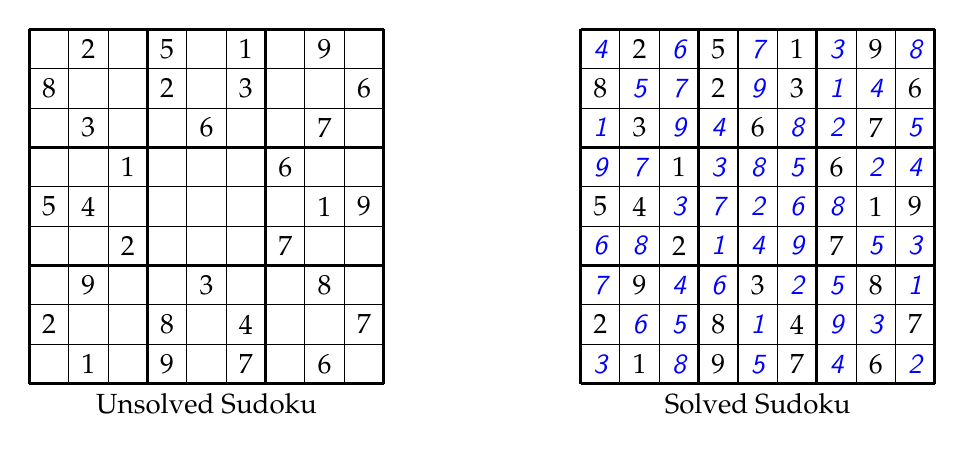
\begin{tikzpicture}[scale=.5]

  \begin{scope}[xshift=-2cm]
    \draw (0, 0) grid (9, 9);
    \draw[very thick, scale=3] (0, 0) grid (3, 3);

    \setcounter{row}{1}
    \setrow { }{2}{ }  {5}{ }{1}  { }{9}{ }
    \setrow {8}{ }{ }  {2}{ }{3}  { }{ }{6}
    \setrow { }{3}{ }  { }{6}{ }  { }{7}{ }

    \setrow { }{ }{1}  { }{ }{ }  {6}{ }{ }
    \setrow {5}{4}{ }  { }{ }{ }  { }{1}{9}
    \setrow { }{ }{2}  { }{ }{ }  {7}{ }{ }

    \setrow { }{9}{ }  { }{3}{ }  { }{8}{ }
    \setrow {2}{ }{ }  {8}{ }{4}  { }{ }{7}
    \setrow { }{1}{ }  {9}{ }{7}  { }{6}{ }

    \node[anchor=center] at (4.5, -0.5) {Unsolved Sudoku};
  \end{scope}

  \begin{scope}[xshift=12cm]
    \draw (0, 0) grid (9, 9);
    \draw[very thick, scale=3] (0, 0) grid (3, 3);

    \setcounter{row}{1}
    \setrow { }{2}{ }  {5}{ }{1}  { }{9}{ }
    \setrow {8}{ }{ }  {2}{ }{3}  { }{ }{6}
    \setrow { }{3}{ }  { }{6}{ }  { }{7}{ }

    \setrow { }{ }{1}  { }{ }{ }  {6}{ }{ }
    \setrow {5}{4}{ }  { }{ }{ }  { }{1}{9}
    \setrow { }{ }{2}  { }{ }{ }  {7}{ }{ }

    \setrow { }{9}{ }  { }{3}{ }  { }{8}{ }
    \setrow {2}{ }{ }  {8}{ }{4}  { }{ }{7}
    \setrow { }{1}{ }  {9}{ }{7}  { }{6}{ }

    \node[anchor=center] at (4.5, -0.5) {Solved Sudoku};

    \begin{scope}[blue, font=\sffamily\slshape]
      \setcounter{row}{1}
      \setrow {4}{ }{6}  { }{7}{ }  {3}{ }{8}
      \setrow { }{5}{7}  { }{9}{ }  {1}{4}{ }
      \setrow {1}{ }{9}  {4}{ }{8}  {2}{ }{5}

      \setrow {9}{7}{ }  {3}{8}{5}  { }{2}{4}
      \setrow { }{ }{3}  {7}{2}{6}  {8}{ }{ }
      \setrow {6}{8}{ }  {1}{4}{9}  { }{5}{3}

      \setrow {7}{ }{4}  {6}{ }{2}  {5}{ }{1}
      \setrow { }{6}{5}  { }{1}{ }  {9}{3}{ }
      \setrow {3}{ }{8}  { }{5}{ }  {4}{ }{2}
    \end{scope}

  \end{scope}

\end{tikzpicture}
\caption{An Example Sudoku Puzzle}
\end{center}
\end{figure}

Given the nature of the problem, solving Sudoku puzzles can easily be modelled as many different constraint satisfaction problems, such as exact cover or boolean satisfiability. In doing so, standard techniques for solving these well known problems can be applied rather than creating a customized solution.  \\

\section{Sudoku as an Exact Cover Problem}
Given a binary matrix, the exact cover problem is to find a set of rows such that there is a 1 in every column in exactly one of the rows in the set. Typically, the columns are used to represent constraints that must be satisfied. Each row in the matrix represents a partial solution, with conflicting partials solutions containing in the same column of their rows for the rule(s) on which they conflict. \\

Sudoku has four types of constraints
\begin{description}
\item[Cell Constraints] Each cell must have exactly one number in it
\item[Row Constraints] Each row much contain each number exactly once
\item[Column Constraints] Each column much contain each number exactly once
\item[Block Constraints] Each block much contain each number exactly once
\end{description}
As such, the base set of constraints result in $4*9*9$ columns; there is a cell constraint for each of the 81 cells and there is a row, column and block constraint for each number in each row, column or block. Furthermore, there are $9*9*9$ rows, one for each number in each cell. The rows have 1's in the columns for the constraints that they satisfy. \\

Once the initial constraints have been set up, the columns all of the constraints which are satisfied by any of given cells in a puzzle can be removed, as well as all rows that could have satisfied any of those constraints. The remaining columns will be those which need to be satisfied in order to complete the puzzle and the rows will be the possible options.
\section{Algorithm X and Dancing Links}
In his paper, "Dancing Links", Donald Knuth describes an algorithm for solving the exact cover problem, which he calls Algorithm X, and a possible implementation technique, which he calls dancing links. This implementation is often referred to as DLX for short. \\
The dancing links approach is based on the observation that an element, x, in a doubly linked list can be removed in the following manner
\[ x.left.right \gets x.right, x.right.left \gets x.left \]
and, more interestingly, x can be re-inserted into the list thusly
\[ x.left.right \gets x, x.right.left \gets x \]
\\
The matrix of the exact cover problem can be represented as a 2-dimensional, circular linked list with a node for every 1 in the matrix, with every node having up, down, left and right pointers. Knuth also uses a set of column header nodes that keep track of additional information about a given column as well as a special \textit{h} node that simply points to the top of the first column. Furthermore, every node has a reference to its column header. This is data structure is shown in Figure~\ref{dlx}. In the figure, the columns are labelled A through G and the numbers below the labels simply refer the number of rows in that column.
\begin{figure}[H]
\begin{center}
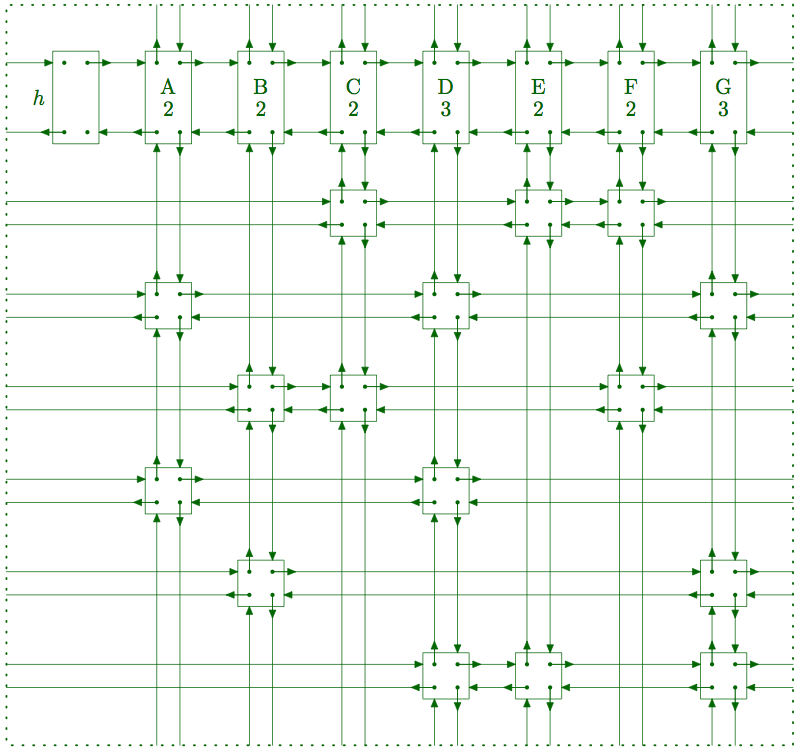
\includegraphics[width=0.9\columnwidth]{dancing_links}
\caption{DLX data structure}
\label{dlx}
\end{center}
\end{figure}
Given this data structure, it is very easy to remove columns and rows, as well as to add them back in again, using the approach described above. The only constraint is that the columns/rows must be added back in in the opposite order from which that in which they were removed. With this in mind, Algorithm X becomes quite simple. \\ 
\begin{algorithm}[H]
\caption{DLX}\label{search}
\begin{algorithmic}[1]
\Procedure{Search}{h: Node}
\If {$h.right = h$}
\State print \textit{solution}
\State \Return
\EndIf
\State $col \gets$ \Call{chooseNextColumn}{$h$}
\State \Call{cover}{$col$}
\ForAll{$row \gets col.down, col.down.down, \dots, while\ row \neq col$}
\State add $row$ to current solution
\ForAll{$j \gets row.right, row.right.right,\dots, while\ j \neq row$}
\State \Call{cover}{$j.colHeader$}
\EndFor
\State \Call{search}{$h$}
\ForAll{$j \gets row.left, row.left.left,\dots, while\ j \neq row$}
\State \Call{uncover}{$j.colHeader$}
\EndFor
\State remove $row$ from the current solution
\EndFor
\State \Call{uncover}{$col$}
\EndProcedure
\end{algorithmic}
\end{algorithm}


The idea is quite simple; we select a column that we want to satisfy and remove it and then, for each row that satisfies the chosen column, we try removing it and all other columns that it satisfies and then we recurse. When the recursion completes, we must undo what we have done so far before we move on to the next candidate row. \\ 

The order in which the columns are chosen does not affect the final result. However, the amount of branching can be reduced if the column with the fewest number of rows is selected at each step. \\

The operation of ``covering'' is also fairly straight forward. We must simply remove the column header from list, so that it will not be chosen later, and then all the rows in the column from all other columns in which they appear. Uncovering, of course, is simply the exact opposite process, done in reverse order. \\

\begin{algorithm}[!ht]
\label{cover}
\begin{algorithmic}
\Procedure{Cover}{col: Node}
\State $col.right.left \gets col.left$
\State $col.left.right \gets col.right$
\ForAll{$row \gets col.down, col.down.down, \dots, while\ row \neq col$}
\ForAll{$j \gets row.right, row.right.right,\dots, while\ j \neq row$}
\State $j.up.down \gets j.down$
\State $j.down.up \gets j.up$
\State $j.colHeader.size \gets j.colHeader.size - 1$
\EndFor
\EndFor
\EndProcedure
\end{algorithmic}
\end{algorithm}

\begin{algorithm}[!ht]
\label{uncover}
\begin{algorithmic}
\Procedure{uncover}{col: Node}
\ForAll{$row \gets col.up, col.up.up, \dots, while\ row \neq col$}
\ForAll{$j \gets row.left, row.left.left,\dots, while\ j \neq row$}
\State $j.up.down \gets j$
\State $j.down.up \gets j$
\State $j.colHeader.size \gets j.colHeader.size + 1$
\EndFor
\EndFor
\State $col.right.left \gets col$
\State $col.left.right \gets col$
\EndProcedure
\end{algorithmic}
\end{algorithm}

\section{Sudoku as a SAT Problem}
The boolean satisfiability problem, SAT, involves finding a satisfying assignment for a boolean expression. These expressions are, typically, written in conjunctive normal form, CNF, i.e. a conjunction of a set of disjunctive clauses. As this is a very well understood problem, there are a wide array of efficient SAT solvers that can be used to solve problems that can be represented as a SAT problem, such as Sudoku. \\

Similar to the exact cover problem, Sudoku lends itself well to being represented as a SAT problem. In order for a CNF expression to be satisfied, each clause must be satisfied, and in order of a clause to be satisfied, one of its literals must be true. As such, we can create a clause for each constraint, made up of literals that represent all of the possible ways to satisfy this constraint. However, we need to be careful to ensure that we do not end up with conflicting literals both being set to True in a satisfying assignment. This can be accomplished by carefully picking which constraints are used or by simply including all possible constraints. \\

The variables of a Sudoku are simply the entries in each of the cells. As such, there must be a variable $s_{xyz} \forall x,y,z \in [1,9]$ where $x$ is a row, $y$ is a column and $z$ is the value in the cell which lies in both row $x$ and column $y$. With this, we can build us clauses for each of the 4 necessary constraints. \\

\begin{description}
\item[Every cell has at least one number] \hfill \\ \\
$\bigwedge\limits_{x=1}^{9} \bigwedge\limits_{y=1}^{9} \bigvee\limits_{z=1}^{9} s_{xyz}$
\item[Each number appears at most once in each row] \hfill \\ \\
$\bigwedge\limits_{y=1}^{9} \bigwedge\limits_{z=1}^{9} \bigwedge\limits_{x=1}^{8} \bigwedge\limits_{i=x+1}^{9}  (\overline{s_{xyz}} \vee \overline{s_{iyz}})$
\item[Each number appears at most once in each column] \hfill \\ \\
$\bigwedge\limits_{x=1}^{9} \bigwedge\limits_{z=1}^{9} \bigwedge\limits_{y=1}^{8} \bigwedge\limits_{i=y+1}^{9}  (\overline{s_{xyz}} \vee \overline{s_{xiz}})$
\item[Each number appears at most once in each block] \hfill \\ \\
$\bigwedge\limits_{z=1}^{9} \bigwedge\limits_{i=0}^{2} \bigwedge\limits_{j=0}^{2} \bigwedge\limits_{x=1}^{3} \bigwedge\limits_{y=1}^{2} \bigwedge\limits_{k=y+1}^{3} (\overline{s_{(3i+x)(3j+y)z}} \vee \overline{s_{(3i+x)(3j+k)z}})$ \\

$\bigwedge\limits_{z=1}^{9} \bigwedge\limits_{i=0}^{2} \bigwedge\limits_{j=0}^{2} \bigwedge\limits_{x=1}^{2} \bigwedge\limits_{y=1}^{3} \bigwedge\limits_{k=x+1}^{3} \bigwedge\limits_{l=1}^{3} (\overline{s_{(3i+x)(3j+y)z}} \vee \overline{s_{(3i+k)(3j+l)z}})$
\end{description}

The above constraints are all that is necessary. However, each of these constraints has an inverse constraint that could also be added, which may or may not allow a SAT solver to eliminate clauses more quick and, thus, solve the puzzle more quickly.

\begin{description}
\item[Every cell has at most one number] \hfill \\ \\
$\bigwedge\limits_{x=1}^{9} \bigwedge\limits_{y=1}^{9} \bigvee\limits_{z=1}^{8} \bigvee\limits_{i=z+1}^{9} (\overline{s_{xyz}} \vee \overline{s_{xyi}})$
\item[Each number appears at least once in each row] \hfill \\ \\
$\bigwedge\limits_{y=1}^{9} \bigwedge\limits_{z=1}^{9} \bigvee\limits_{x=1}^{9}   s_{xyz}$
\item[Each number appears at least once in each column] \hfill \\ \\
$\bigwedge\limits_{x=1}^{9} \bigwedge\limits_{z=1}^{9} \bigvee\limits_{y=1}^{9} s_{xyz}$
\item[Each number appears at least once in each block] \hfill \\ \\
$\bigwedge\limits_{z=1}^{9} \bigwedge\limits_{i=0}^{2} \bigwedge\limits_{j=0}^{2} \bigwedge\limits_{x=1}^{3} \bigwedge\limits_{y=1}^{3} s_{(3i+x)(3j+y)z}$
\end{description}
The first 4 sets of constraints listed are usually known as the ``minimal encoding'' while the set of all 8 constraints is known as the ``extended encoding''. After all the constraint clauses are added, for either the minimal or extended encoding, we must then add clauses for each of the given elements in the initial grid. This clauses will only contain one literal, corresponding to the number and the row and column it appears in, forcing that variable to be true in any satisfying assignment.

\section{Generating Sudoku Puzzles}
In order to evaluate the different methods for solving Sudoku puzzles, a large set of puzzles is necessary for testing. Thankfully, the nature of the DLX algorithm makes it perfect for both solving and generating Sudoku puzzles. Given an empty starting grid, DLX will eventually generate all possible completed Sudoku puzzles. In order to randomize this process, so as to not generate a set of puzzles that are all closely related, we need only to randomize the order in which rows are selected at line 7 in Algorithm \ref{search}. The column selection need not be randomized as all columns must be selected at some point before a valid solution is found. The order in which the rows are selected, however, define which way each constraint is satisfied. \\

In order to speed up the process slightly, a random permutation of 1~9 can be placed in the first row without needing to do any validation. The same idea can be applied to filling in the first column and the first block, by simply permuting the remaining available numbers. However, this process is not necessary for the algorithm to be able to generate a random puzzle.\\

After a completed grid is generated, we must remove a certain number of clues. A valid Sudoku puzzle must only have one solution so a good strategy is to simply try removing each of the clues, i.e. currently filled-in cells, in a random order, testing to ensure that the puzzle still has only one solution at each step and replacing the clue if it has more than one. This can easily be accomplished using DLX as it is able to easily determine the number of possible solutions. \\

This approach typically results in very difficult puzzles being generated. In order to get around, one could add back in clues until the desired difficulty is reached. However, this would require creating a system that can determine the difficulty of a Sudoku puzzle which would involve emulating the ways in which humans solve the puzzles. This was not necessary for the project, however, as difficult puzzles are a good test of the efficiency of solving algorithms.

\section{Implementation}
All source code is available on \href{https://github.com/smaskell/Sudoku}{GitHub}.
\subsection{Sudoku Generation}
In order to generate Sudoku puzzles, the Algorithm X was implemented in Python. This allowed for the algorithm to use of Python's generator construct. With this mechanic, the algorithm is very easily able to generate solutions to a given puzzle one at a time on demand, rather than generating all of them all at once, which is would be incredibly slow in the generation phase. \\

A noted by Ali Assaf of McGill University, Algorithm X can be very easily and succinctly implemented in python by using two dictionary objects, one which maps a column name to a set of rows and one which does the opposite. Dictionary and set objects in Python constant time insertion and deletion methods which means that Algorithm X can be efficiently implemented using a very similar technique to dancing links. The dictionary and set data structure, however, allows for much simpler problem set-up. Furthermore, it is much simpler to permute a set in order to pick rows in a random order than it is to do so with a linked list. This makes the random generation process  very straightforward.\\

\subsection{Sudoku Solving}
\subsubsection{DLX}
In order to truly test the efficiency of DLX on a Sudoku problem, Python is not a very suitable language as it requires much overhead. As such, DLX was implemented in C++, using structs to represent the nodes of the linked list. This implementation followed Knuth's description very closely. As the Sudoku generator was implemented using Algorithm X, it is capable of converting a Sudoku problem into an exact cover problem so it is used to do so. This representation of the problem is then written to standard out so that it can be read by the C++ program, which simply writes a list of row numbers of the solution to standard out. Unlike the Python implementation, the C++ version generates all possible solutions to a given puzzle every time. However, since it is only used on valid Sudoku puzzles that only have one solution, this is not much of an issue. \\

As each row represents a certain digit being placed in a certain cell, it is very easy to map the result DLX, a list of rows, back to the Sudoku problem. One must simply fill in the cells that correspond to the rows in the solution to the exact cover problem in order to find the solution to the Sudoku puzzle.

\subsubsection{SAT}
As the Sudoku puzzles are generated in Python, another script for converting puzzles to SAT format was also written in Python. This conversion script is based heavily on the work done by Binnersley, Maskell and Simas. This converted form is then written to standard out so that it can be read by a SAT solver. A collection of Knuth's SAT solvers, including SAT0W, SAT9 and SAT10, was used for solving the resulting SAT problem. \\

Each variable in the SAT problem correspond to a specific digit being placed in a certain cell. As such, one can find the solution to the Sudoku puzzle by filling in the cells corresponding to all of the unbarred literals in the satisfying assignment.

\section{Results}
Five hundred Sudoku puzzles were generated using the techniques described earlier. These were then converted to exact cover format and SAT, using both minimal and extended encodings. DLX and Knuth's SAT solver were then tested on the results. The average running times across the five hundred puzzles is listed in Table-\ref{table:runningtime}

\begin{table}[H]
\begin{center}
\begin{tabular}{cccc}
DLX - All solutions & DLX - Single Solution & SAT13 - Minimal & Sat13 - Extended\\
0.08678 & 0.085526 & 0.00628 & 0.007316
\end{tabular}
\caption{Average running time in seconds of the tested algorithms}
\label{table:runningtime}
\end{center}
\end{table}

Surprisingly, Knuth's SAT solver performed much better than DLX. However, it is clear than much time has been spent optimizing SAT13 so it is possible that better results could be achieved with DLX if it were to be optimized further. This is illustrated very clearly by the fact that some of Knuth's earlier SAT solvers, such as SAT10 and SAT0W, were also tested but were far too slow to complete the test set in any reasonable amount of time, taking many minutes to solve certain inputs. \\

Another surprising revelation is that DLX had almost identical performance whether it stopped after finding the first solution or not. This is most likely due to the fact that simply reading the input and building the data structure is the most expensive operation, and this is not affected by the change. If this process could be optimized, the algorithm would, most likely, run much faster. \\

SAT13 performed very well on both the minimal and extended encoding, though the minimal encoding gave better results. This is likely due to the fact that reading in the extended encoding and building the data structures takes much longer, as the input is roughly twice the size of the minimal encoding. 
\section{Conclusion}
Given the nature of the Sudoku problem, it is very easy to map it to other constraint satisfaction problems. This allows for the use of well known algorithms such as DLX or certain SAT solving algorithms. Both of these approaches performed quite well, though Knuth's SAT13 yielded the best results. DLX, if slightly slower, however, is still ideal for Sudoku generation as it is able to easily generate all possible solutions to a Sudoku puzzle, rather than simply stopping after finding the first one.
\end{document}